\documentclass[12pt, twoside]{article}
\usepackage[letterpaper, margin=1in, headsep=0.5in]{geometry}
\usepackage[english]{babel}
\usepackage[utf8]{inputenc}
\usepackage{amsmath}
\usepackage{amsfonts}
\usepackage{amssymb}
\usepackage{tikz}
%\usetikzlibrary{quotes, angles}

\usepackage{graphicx}
\usepackage{enumitem}
\usepackage{multicol}

\usepackage{fancyhdr}
\pagestyle{fancy}
\fancyhf{}
\renewcommand{\headrulewidth}{0pt} % disable the underline of the header

\fancyhead[LE]{\thepage}
\fancyhead[RO]{\thepage \\ Name: \hspace{4cm} \,\\}
\fancyhead[LO]{BECA / Dr. Huson / Geometry\\* Unit 7: Similarity\\* 9 January 2020}

\begin{document}
\subsubsection*{7.6 Homework: Similarity transformations and the tangent function}
  \begin{enumerate}

  \item Triangle $ABC$ is dilated with a factor of $\frac{5}{4}$ centered at $A$, yielding $\triangle ADE$, as shown. Given $AB=8$, $BC=12$, and $AC=14$. \\[0.25cm] Find $BD$, $AE$, and $DE$. \vspace{1cm}
  \begin{flushright}
      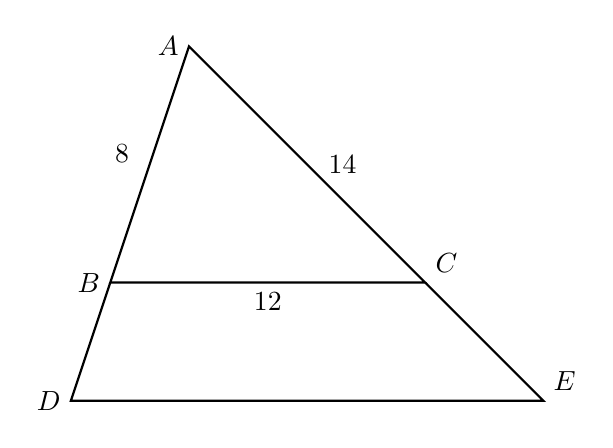
\begin{tikzpicture}[scale=0.5]
        \draw [thick]
        (0,0)node[left]{$B$}--
        (8,0)node[above right]{$C$}--
        (2,6)node[left]{$A$}--cycle;
        \draw [thick]
        (0,0)--
        (-1,-3)node[left]{$D$}--
        (11,-3)node[above right]{$E$}--(8,0);
        \node at (4,0)[below]{$12$};
        \node at (5.3, 3)[right]{$14$};
        \node at (0.3, 2.8)[above]{$8$};
      \end{tikzpicture}
    \end{flushright}

  \item The vertices of $\triangle JKL$ have the coordinates $J(-4,-2)$, $K(4,2)$, and $L(-2,4)$, as shown. \\[0.25cm]
  Apply a dilation to $\triangle JKL \rightarrow \triangle J'K'L'$, centered on the origin and with a scale factor $k=1.5$. Draw the image $\triangle J'K'L'$ on the set of axes below, labeling the vertices, and make a table showing the correspondence of both triangles' coordinate pairs.
    \begin{flushright}
      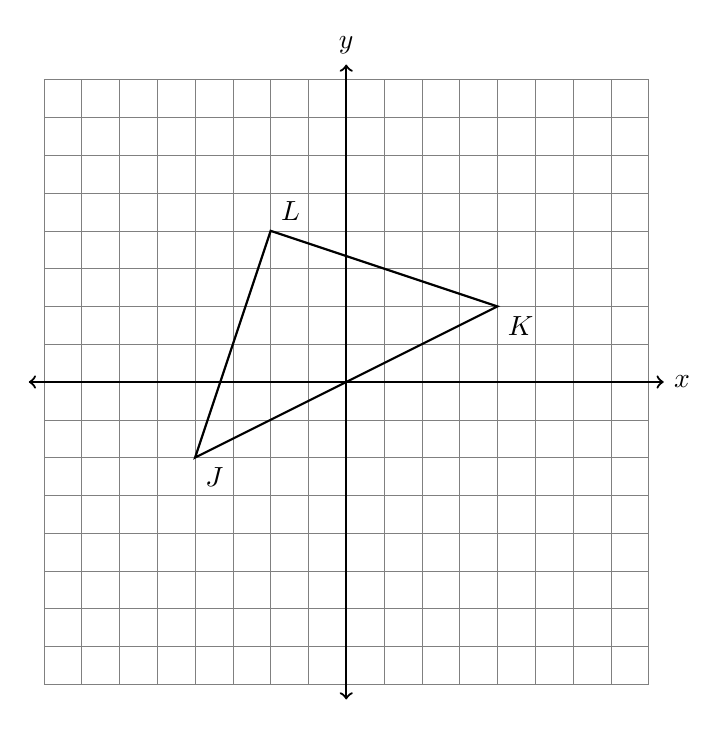
\begin{tikzpicture}[scale=.48]
        \draw [help lines] (-8,-8) grid (8,8);
        \draw [thick, <->] (-8.4,0) -- (8.4,0) node [right] {$x$};
        \draw [thick, <->] (0,-8.4)--(0,8.4) node [above] {$y$};

        \draw [thick]
        (-4,-2) node[below right] {$J$}--
        (4,2) node[below right] {$K$}--
        (-2,4) node[above right] {$L$}--
        cycle;
      \end{tikzpicture}
    \end{flushright}

\newpage
  \item What is the smallest non-zero angle of rotation about its center that would map the octagon onto itself? \vspace{0.25cm}
  \begin{center}
      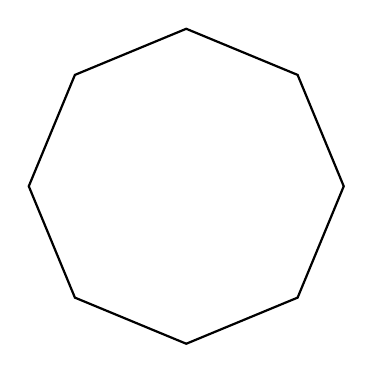
\begin{tikzpicture}%[scale=.48]
        \draw [thick]
        (0:2)--
        (45:2)--
        (90:2) --
        (135:2)--
        (180:2)--
        (225:2)--
        (270:2)--
        (315:2)--cycle;
      \end{tikzpicture}
    \end{center}

  \item The vertices of $\triangle JKL$ have the coordinates $J(-4,-2)$, $K(-1,-1)$, and $L(-2,3)$, as shown below. \\[0.5cm]
  Apply a translation of $(x,y) \rightarrow (x-3, y+2)$ to $\triangle JKL$ and then reflect the image across the $y$-axis. Draw both images $\triangle J'K'L'$ and $\triangle J''K''L''$ on the set of axes below, labeling the vertices.  \vspace{3cm}
  \begin{center}
    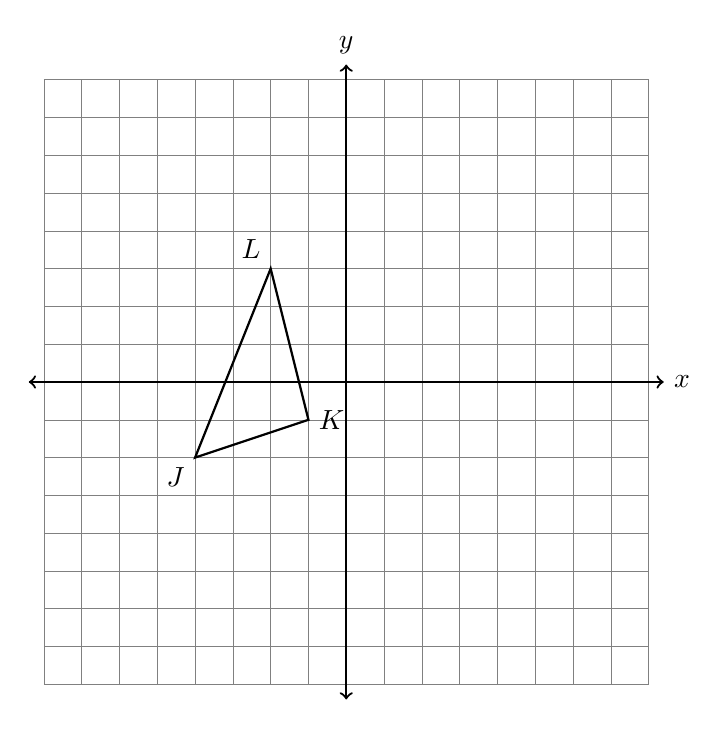
\begin{tikzpicture}[scale=.48]
      \draw [help lines] (-8,-8) grid (8,8);
      \draw [thick, <->] (-8.4,0) -- (8.4,0) node [right] {$x$};
      \draw [thick, <->] (0,-8.4)--(0,8.4) node [above] {$y$};

      \draw [thick]
      (-4,-2) node[below left] {$J$}--
      (-1,-1) node[right] {$K$}--
      (-2,3) node[above left] {$L$}--
      cycle;
    \end{tikzpicture}
  \end{center}

\end{enumerate}
\end{document}